\section{Lenses, packages and directional audits}
\label{sec:sbt-framework}

This section introduces the few Six Birds / SBT notions we need \cite{sixbirds_foundations,sixbirds_darkenergy} and defines the audit statistic used throughout. The framework supplies vocabulary and a checklist. The quantitative content of the paper lies in the statistics defined here and in the mathematics of \cref{sec:boundary-mode}.

\paragraph{Lenses, completions and packages.}
Let $X$ denote the underlying state: the cosmology together with instrumental, calibration and foreground degrees of freedom. A \emph{lens} is a data-processing and compression map
\begin{equation}
  \Lens : X \to \mathcal{L},
  \label{eq:lens_map}
\end{equation}
which ends in a likelihood object. In this paper a lens is a released likelihood, such as SPT-3G 2018 or SPT-3G D1. A \emph{completion} $\Completion$ supplies what the lens leaves open: here the $\Lambda$CDM$+\mnu$ model with three degenerate massive neutrinos, the physical gate $\mnu\ge0$, each release's own nuisance model and priors, and any external data held fixed (for example DESI BAO). The reported inference, a posterior or a best fit, is the \emph{package}
\begin{equation}
  \Pack \;=\; \Completion\circ\Lens .
  \label{eq:packaging_def}
\end{equation}
If two lenses view the same sky coherently, swapping one for the other should not drastically change the package. When the package does change, SBT asks two questions before any physical interpretation: do the lenses predict each other, and does the change survive controls on staging (cuts, support, resolution)?

\paragraph{The directional audit.}
Let $\log\mathcal{L}_A$ and $\log\mathcal{L}_B$ be the log-likelihoods of lenses $A$ and $B$, each including the common completion, as functions of a parameter vector $\theta$. Let $\hat\theta_A$ and $\hat\theta_B$ be best fits. The mismatch of $B$ given $A$ is
\begin{equation}
  \dchi_{B|A} \;\equiv\; -2\left[\log \mathcal{L}_B(\hat\theta_A) - \log \mathcal{L}_B(\hat\theta_B)\right].
  \label{eq:dchi_def}
\end{equation}
It measures how much worse $B$ fits at parameters chosen by $A$ than at its own best fit. Two properties matter.

\begin{itemize}[leftmargin=*, itemsep=2pt]
  \item \emph{Sign.} $\dchi_{B|A}\ge0$ holds whenever $\log\mathcal{L}_B(\hat\theta_B)\ge\log\mathcal{L}_B(\hat\theta_A)$. A global maximum over a domain that contains $\hat\theta_A$ guarantees this, but an optimizer reporting success does not. In practice we start the reference fit from the transferred point and keep the better of the two, so the ordering holds between the retained points, without any claim that the global maximum has been found. (Lean: Appendix~\ref{app:formal}, \texttt{Audit}.)
  \item \emph{Direction.} In general $\dchi_{B|A}\ne\dchi_{A|B}$. The two lenses have different noise, multipole coverage and nuisance freedom, so ``how well 2018 predicts D1'' and ``how well D1 predicts 2018'' are different questions. We always report both.
\end{itemize}

In practice the two lenses share only some parameters. We write $\theta=(\phi,\eta_B)$, where $\phi$ are the shared parameters transferred from the train fit and $\eta_B$ are nuisance parameters of the test lens that are re-fitted (profiled). The audit then compares the profiled likelihood $\max_{\eta_B}\log\mathcal{L}_B(\hat\phi_A,\eta_B)$ with the reference fit of $B$. The statistic is a comparative diagnostic in native $-2\Delta\log\mathcal{L}$ units. It is not a calibrated $p$-value: the two releases differ in seasons, noise and nuisance models, and translating $\dchi$ into a significance would require a declared null distribution, which we do not construct.

\begin{figure}[t]
  \centering
  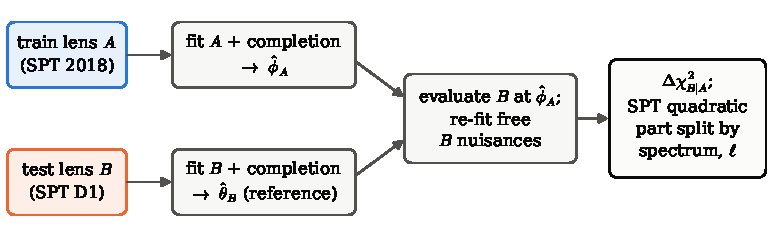
\includegraphics[width=\linewidth]{figures/fig_audit_schema.pdf}
  \caption{The directional audit $\dchi_{B|A}$. Each lens is fitted together with the same completion. The shared parameters $\hat\phi_A$ from the train lens are transferred to the test lens, whose remaining free nuisance parameters (if any) are re-fitted. The loss in fit relative to the test lens's own best fit is recorded; its SPT quadratic part is split over spectra and multipole bands, and native prior and normalization terms are kept as separate ledger entries (\cref{sec:ledger}). Exchanging the roles of $A$ and $B$ gives $\dchi_{A|B}$.}
  \label{fig:audit-schema}
\end{figure}

\paragraph{Staging controls.}
SBT separates genuine disagreement from \emph{staging}: changes in cuts, support or resolution that alter a package even when every component is internally consistent \cite{sixbirds_foundations}. For CMB likelihoods the obvious staging variable is multipole coverage. D1 covers TT down to $\ell=400$ and TE/EE up to $\ell=4000$, which 2018 does not. A support-cut control removes this extra D1 coverage and repeats the audit (\cref{sec:common-staging}). If the mismatch survives, extra support cannot explain it. A support cut does not equalize window functions, binning or resolution, so it tests one specific staging explanation and not all of them.

\paragraph{The six primitives in this setting.}
\Cref{tab:sixbirds_primitives} lists how the six SBT primitives appear here. The table is a reading guide, not an additional result.

\begin{table}[t]
  \centering
  \caption{The six Six Birds primitives and their role in the SPT 2018 $\leftrightarrow$ D1 lens swap.}
  \label{tab:sixbirds_primitives}
  \setlength{\tabcolsep}{4pt}
  \renewcommand{\arraystretch}{1.08}
  \small
  \begin{tabular}{@{}>{\raggedright\arraybackslash}p{0.17\linewidth} >{\raggedright\arraybackslash}p{0.27\linewidth} >{\raggedright\arraybackslash}p{0.50\linewidth}@{}}
    \toprule
    Primitive & Informal meaning & Role in this work \\
    \midrule
    \textbf{P1 Rewrite} & Minimal correction that restores consistency of a package &
    Not applied to the SPT data. A toy template projection (Appendix~\ref{app:reproducibility}) reduces a fitted residual by construction; this is descriptive fit improvement, not evidence of predictive repair. \\
    \textbf{P2 Gating} & Constraints defining admissible objects &
    Physical gate $\mnu\ge0$; finite prior box $\mnu\le5$\,eV; choice of included likelihoods. \\
    \textbf{P3 Route mismatch} & Packages that depend on the route taken &
    The 2018 and D1 lenses give different packages; quantified by $\dchi_{B|A}$ and $\dchi_{A|B}$. \\
    \textbf{P4 Staging} & Dependence on cuts, support, resolution &
    Support-cut control removing D1's extra multipole coverage. \\
    \textbf{P5 Packaging} & The package $\Completion\circ\Lens$ &
    $\mnu$ posteriors and best fits, together with nuisance and native priors (including each release's own optical-depth prior). \\
    \textbf{P6 Audit} & Held-out prediction and accounting &
    Directional audits and exact signed localization by spectrum and multipole. \\
    \bottomrule
  \end{tabular}
\end{table}
